\chapter{लाग्रांजियन यांत्रिकी}\label{ch:b3:lagrangian-mechanics}

किसी द्विक लोलक के लिए न्यूटन का नियम लिखकर देखिए: दो तनाव-बल, जिनमें
से एक भी पहले से ज्ञात नहीं, दोनों हर क्षण दिशा बदलते हुए, और केवल यह
जानने के लिए कि दो कोण कैसे विकसित होते हैं, चार अदिश समीकरण सुलझाने
पड़ते हैं। अब वही काम किसी घूमते वलय पर पिरोए मनके के लिए कीजिए, युग्मित
स्प्रिंगों की शृंखला के लिए, किसी यंत्र-भुजा के लिए। जो बल तंत्र को
बाँधे रखते हैं --- छड़ें, पटरियाँ, कब्ज़े --- वे कोई कार्य नहीं करते,
फिर भी न्यूटन की विधि हमें उन्हें हर गणना में ढोने पर विवश करती है। यह
अध्याय वह पुनर्रचना प्रस्तुत करता है जो लाग्रांज ने 1788 में प्रकाशित
की: तंत्र का वर्णन उन थोड़े-से निर्देशांकों से कीजिए जो वास्तव में बदल
सकते हैं, एक अकेला फलन $L = E_k - E_p$ लिखिए, और एक ही विधि किन्हीं भी
निर्देशांकों में गति के समीकरण दे देती है, जिनमें हर छड़ और हर पटरी पहले
ही लुप्त हो चुकी है। इससे भी बढ़कर, नई रचना वह उजागर कर देती है जिसे
न्यूटन की रचना छिपा जाती है: $L$ की हर सममिति से एक संरक्षित राशि निकलती
है --- स्थान की एकरूपता से संवेग, समय की एकरूपता से ऊर्जा --- एमी नोएटर
का यह परिणाम यांत्रिकी से कहीं आगे बढ़कर भौतिकी का संगठक सिद्धांत बन
चुका है।

\section{बलों से निर्देशांकों तक}

\begin{definition}[प्रतिबंध, स्वातंत्र्य कोटि, व्यापकीकृत निर्देशांक]\label{def:b3:lagrangian-mechanics:coordinates}
\index{प्रतिबंध}\index{स्वातंत्र्य कोटि}\index{व्यापकीकृत निर्देशांक}
\emph{प्रतिबंध} किसी तंत्र की स्थितियों पर लगी ज्यामितीय शर्त है ---
मनका अपने तार पर बना रहता है, लोलक की छड़ की लंबाई नियत रहती है, एक ही
धुरी के दो पहिये साथ-साथ घूमते हैं। जो प्रतिबंध निर्देशांकों (और संभवतः
समय) के बीच किसी समीकरण
$f(\vect r_1, \dots, \vect r_N, t) = 0$ के रूप में लिखा जा सके, उसे
\emph{होलोनॉमिक} कहते हैं। विन्यास जितने स्वतंत्र तरीकों से अब भी बदल
सकता है, उनकी संख्या ही \emph{स्वातंत्र्य कोटि} की संख्या $n$ है; ऐसी
कोई भी $n$ स्वतंत्र राशियाँ $q_1, \dots, q_n$, जो विन्यास को पूरी तरह
नियत कर दें, \emph{व्यापकीकृत निर्देशांक} कहलाती हैं --- कोण, लंबाइयाँ,
या दोनों का कोई सुविधाजनक मिश्रण। इनके समय-अवकलज
$\dot q_1, \dots, \dot q_n$
\emph{व्यापकीकृत वेग}\index{व्यापकीकृत वेग} हैं।
\end{definition}

\begin{example}[स्वातंत्र्य कोटि गिनना]\label{ex:b3:lagrangian-mechanics:counting}
मेज़ पर एक बिंदु: $n = 2$। नियत लंबाई का समतलीय लोलक: एक कोण,
$n = 1$। द्विक लोलक: दो कोण, $n = 1 + 1 = 2$। दृढ़ वलय पर पिरोया मनका:
एक कोण, $n = 1$ --- चाहे वलय स्वयं घूमने पर विवश हो, क्योंकि आरोपित
घूर्णन कोई स्वतंत्रता नहीं जोड़ता। अंतरिक्ष में स्वतंत्र दृढ़ पिंड: उसके
केंद्र के तीन निर्देशांक और तीन कोण, $n = 6$। $N$ स्वतंत्र अणुओं
(बिंदुओं) की गैस: $n = 3N$। हर होलोनॉमिक
\omterm{def:b3:lagrangian-mechanics:coordinates}{प्रतिबंध} एक \omterm{def:b3:lagrangian-mechanics:coordinates}{स्वातंत्र्य कोटि} घटा देता है: छड़ से जुड़े दो बिंदुओं के लिए
$3 + 3 - 1 = 5$।
\end{example}

\begin{omfigure}
\begin{tikzpicture}[font=\small, >=Stealth]
  % (a) plane pendulum
  \begin{scope}
    \draw[thick] (-1,0) -- (1,0);
    \foreach \i in {-0.8,-0.5,-0.2,0.1,0.4,0.7} \draw (\i,0) -- (\i+0.18,0.16);
    \fill (0,0) circle (1.5pt);
    \draw[dashed] (0,0) -- (0,-2.2);
    \draw[thick] (0,0) -- (-55:2.1);
    \fill[omDef] (-55:2.1) circle (3pt);
    \draw[->] (0,-1.0) arc (-90:-55:1.0);
    \node at (-72:1.35) {$\theta$};
    \node at (-55:2.5) {$m$};
    \node at ($(-55:1.35)+(0.28,0.12)$) {$\ell$};
    \node at (0,-2.9) {एक निर्देशांक: $\theta$};
  \end{scope}
  % (b) bead on rotating hoop
  \begin{scope}[xshift=6.2cm]
    \coordinate (C) at (0,-2.35);
    \draw[thick] (C) circle (1.55);
    \draw[dashed] (0,-0.3) -- (0,-4.6);
    \draw[->, thick] (0.35,-0.15) arc (20:160:0.37);
    \node at (0,0.25) {$\omega$};
    \fill (C) circle (1pt);
    \draw (C) -- ++(-50:1.55);
    \fill[omDef] ($(C)+(-50:1.55)$) circle (3pt);
    \draw[->] ($(C)+(0,-0.85)$) arc (-90:-50:0.85);
    \node at ($(C)+(-70:1.18)$) {$\theta$};
    \node at ($(C)+(-38:2.0)$) {$m$};
    \draw (C) -- ++(135:1.55);
    \node at (-1.35,-1.35) {$R$};
    \node at (0,-4.95) {एक निर्देशांक: $\theta$};
  \end{scope}
  % (c) double pendulum
  \begin{scope}[xshift=11.4cm]
    \draw[thick] (-0.9,0) -- (0.9,0);
    \foreach \i in {-0.7,-0.4,-0.1,0.2,0.5} \draw (\i,0) -- (\i+0.18,0.16);
    \fill (0,0) circle (1.5pt);
    \draw[dashed] (0,0) -- (0,-1.7);
    \draw[thick] (0,0) -- (-65:1.5) coordinate (m1);
    \fill[omDef] (m1) circle (2.6pt);
    \draw[dashed] (m1) -- ++(0,-1.5);
    \draw[thick] (m1) -- ++(-40:1.5) coordinate (m2);
    \fill[omThm] (m2) circle (2.6pt);
    \draw[->] (0,-0.8) arc (-90:-65:0.8);
    \node at (-80:1.1) {$\theta_1$};
    \draw[->] ($(m1)+(0,-0.75)$) arc (-90:-40:0.75);
    \node at ($(m1)+(-68:1.05)$) {$\theta_2$};
    \node at (0.3,-3.4) {दो निर्देशांक: $\theta_1, \theta_2$};
  \end{scope}
\end{tikzpicture}

{\small \omterm{def:b3:lagrangian-mechanics:coordinates}{व्यापकीकृत निर्देशांक}: हर तंत्र का वर्णन उन कोणों से किया जाता
है जो वास्तव में बदल सकते हैं, न कि उसके द्रव्यमानों के कार्तीय
निर्देशांकों से। छड़ों के तनाव और वलय का अभिलंब बल कभी प्रकट नहीं होते।}
\end{omfigure}

\section{न्यूनतम क्रिया का सिद्धांत}

\begin{definition}[लाग्रांजियन और क्रिया]\label{def:b3:lagrangian-mechanics:action}
\index{लाग्रांजियन}\index{क्रिया}
किसी ऐसे यांत्रिक तंत्र का \emph{लाग्रांजियन}, जिसके बल किसी स्थितिज
ऊर्जा $E_p$ से व्युत्पन्न होते हैं, निर्देशांकों, वेगों और संभवतः समय
का यह फलन है
\[
L(q, \dot q, t) = E_k - E_p ,
\]
अर्थात् गतिज ऊर्जा \emph{ऋण} स्थितिज ऊर्जा, दोनों व्यापकीकृत
निर्देशांकों में व्यक्त। किसी कल्पनीय गति $q(t)$ की, जो नियत सिरों
$q(t_1)$ और $q(t_2)$ के बीच चलती है, \emph{क्रिया} वह संख्या है
\[
S[q] = \int_{t_1}^{t_2} L\big(q(t), \dot q(t), t\big)\,\dd t .
\]
$S$ एक \emph{फलनक} है: यह पूरा एक पथ निगलता है और एक संख्या लौटाता है,
जूल-सेकंड में --- प्लांक के नियतांक के मात्रक।
\end{definition}

\begin{theorem}[हैमिल्टन का सिद्धांत और ऑयलर--लाग्रांज समीकरण]\label{thm:b3:lagrangian-mechanics:euler-lagrange}
\index{हैमिल्टन का सिद्धांत}\index{ऑयलर--लाग्रांज समीकरण}\index{न्यूनतम क्रिया}
समान दो सिरों को समान समय में जोड़ने वाली सभी कल्पनीय गतियों में से
वास्तविक गति वही है जो \omterm{def:b3:lagrangian-mechanics:action}{क्रिया} को
\emph{स्थिर} बना देती है (\emph{\omterm{thm:b3:lagrangian-mechanics:euler-lagrange}{हैमिल्टन का सिद्धांत}}, अथवा
\emph{\omterm{thm:b3:lagrangian-mechanics:euler-lagrange}{न्यूनतम क्रिया}} का सिद्धांत)। समतुल्य रूप से, गति
\emph{ऑयलर--लाग्रांज समीकरणों} का पालन करती है
\[
\frac{\dd}{\dd t}\frac{\partial L}{\partial\dot q_i}
 - \frac{\partial L}{\partial q_i} = 0 ,
\qquad i = 1, \dots, n :
\]
प्रत्येक \omterm{def:b3:lagrangian-mechanics:coordinates}{स्वातंत्र्य कोटि} के लिए एक द्वितीय-कोटि समीकरण, चाहे निर्देशांक
कोई भी चुने गए हों।
\end{theorem}

\begin{proof}
पथ को विरूपित कीजिए: $q_i(t) \to q_i(t) + \delta q_i(t)$, जहाँ
$\delta q_i(t_1) = \delta q_i(t_2) = 0$। प्रथम कोटि तक,
\[
\delta S = \int_{t_1}^{t_2}\sum_i\Big(
  \frac{\partial L}{\partial q_i}\,\delta q_i
 + \frac{\partial L}{\partial\dot q_i}\,\delta\dot q_i\Big)\dd t
 = \int_{t_1}^{t_2}\sum_i\Big(
  \frac{\partial L}{\partial q_i}
 - \frac{\dd}{\dd t}\frac{\partial L}{\partial\dot q_i}\Big)\delta q_i\,\dd t ,
\]
दूसरे पद का खंडशः समाकलन करने के बाद ($\delta\dot q_i =
\dd(\delta q_i)/\dd t$) और सीमा-पद छोड़ देने के बाद, जो नियत सिरों पर
लुप्त हो जाता है। यदि \emph{हर} विरूपण के लिए $\delta S = 0$ हो, तो
कोष्ठक को हर क्षण और हर $i$ के लिए शून्य होना ही चाहिए --- यदि वह कहीं
धनात्मक होता, तो वहीं संकेंद्रित एक उभार $\delta q_i$ से
$\delta S \neq 0$ मिल जाता। विलोम उसी पंक्ति से पढ़ लिया जाता है।
\end{proof}

\begin{omfigure}
\begin{tikzpicture}[font=\small, >=Stealth]
  \draw[->] (0,0) -- (7.6,0) node[right] {$t$};
  \draw[->] (0,0) -- (0,3.4) node[above] {$q$};
  \fill (0.8,0.7) circle (2pt) node[below left] {$q(t_1)$};
  \fill (6.8,2.3) circle (2pt) node[above right] {$q(t_2)$};
  \draw[omDef, very thick] (0.8,0.7) .. controls (2.6,2.6) and (5.0,1.4) .. (6.8,2.3);
  \draw[omExo, dashed] (0.8,0.7) .. controls (2.2,0.6) and (5.4,0.9) .. (6.8,2.3);
  \draw[omExo, dashed] (0.8,0.7) .. controls (3.0,3.6) and (5.2,2.9) .. (6.8,2.3);
  \node[omDef] at (1.9,3.35) {वास्तविक पथ};
  \draw[->, omDef] (2.25,3.15) -- (2.85,2.3);
  \node[omExo] at (3.4,0.42) {विचलित पथ};
  \draw[<->] (4.1,1.62) -- (4.1,2.62);
  \node at (4.55,2.15) {$\delta q$};
\end{tikzpicture}

{\small \omterm{thm:b3:lagrangian-mechanics:euler-lagrange}{हैमिल्टन का सिद्धांत}: समान सिरों और समान अवधि वाले सभी पथों में
से वास्तविक पथ $S = \int L\,\dd t$ को स्थिर बनाता है --- प्रथम कोटि के
विरूपण $\delta q$ से $S$ में परिवर्तन केवल द्वितीय कोटि पर होता है।}
\end{omfigure}

\begin{proposition}[न्यूटन की पुनर्प्राप्ति]\label{prop:b3:lagrangian-mechanics:newton}
कार्तीय निर्देशांकों में एक कण के लिए $L = \tfrac12 m(\dot x^2 +
\dot y^2 + \dot z^2) - E_p(x,y,z)$, और \omterm{thm:b3:lagrangian-mechanics:euler-lagrange}{ऑयलर--लाग्रांज समीकरण}
$m\ddot x = -\partial E_p/\partial x$ बन जाते हैं, तथा $y$, $z$ के लिए
भी वैसे ही: ठीक $m\vect a = \vect F$। \omterm{def:b3:lagrangian-mechanics:action}{लाग्रांजियन} और न्यूटनी यांत्रिकी
वहाँ सहमत हैं जहाँ दोनों लागू होती हैं; नया रूप निर्देशांकों का परिवर्तन
झेल जाता है, जो न्यूटन के घटक-समीकरण नहीं झेलते।
\end{proposition}

\begin{proof}
$\partial L/\partial\dot x = m\dot x$, $\partial L/\partial x =
-\partial E_p/\partial x$; \omterm{thm:b3:lagrangian-mechanics:euler-lagrange}{ऑयलर--लाग्रांज समीकरण}
$\dd(m\dot x)/\dd t + \partial E_p/\partial x = 0$ है।
\end{proof}

\begin{remark}[प्रतिबंध-बल क्यों गायब हो जाते हैं]\label{rem:b3:lagrangian-mechanics:constraints}
छड़ का तनाव, पटरी का अभिलंब बल --- ये हर उस विस्थापन के लंबवत लगते हैं
जिसकी \omterm{def:b3:lagrangian-mechanics:coordinates}{प्रतिबंध} अनुमति देता है: \omterm{def:b3:lagrangian-mechanics:coordinates}{प्रतिबंध} के अनुकूल किसी भी गति में वे कोई
कार्य नहीं करते। चूँकि \omterm{def:b3:lagrangian-mechanics:action}{क्रिया} केवल ऐसी ही गतियों पर आँकी गई ऊर्जाओं से
बनी है, इसलिए ये बल $L$ में कभी प्रवेश नहीं करते --- यही इस विधि का
व्यावहारिक चमत्कार है। इसका सामान्य औचित्य (आभासी कार्य का दालंबेर
सिद्धांत) यहाँ स्वीकृत है; इस पुस्तक के हर तंत्र के लिए नीचे दी गई विधि
सीधे न्यूटन के विरुद्ध जाँची जा सकती है, जैसा
\cref{prop:b3:lagrangian-mechanics:newton} ने करना शुरू किया। यदि
प्रतिबंध-बल स्वयं चाहिए हो --- क्या छड़ टूट जाएगी? --- तो गति ज्ञात हो
जाने पर उस अकेले बल के लिए न्यूटन पर लौट आइए।
\end{remark}

\begin{method}[लाग्रांजियन विधि]\label{met:b3:lagrangian-mechanics:recipe}
(1) \omterm{def:b3:lagrangian-mechanics:coordinates}{स्वातंत्र्य कोटि} गिनिए और निर्देशांक $q_i$ चुनिए ---
घूर्णनों के लिए कोण, पटरियों के अनुदिश भुज। (2) स्थितियाँ
$\vect r(q_i, t)$ व्यक्त कीजिए, वेग पाने के लिए अवकलन कीजिए, और
$E_k$ लिखिए; $E_p$ लिखिए। (3) $L = E_k - E_p$, कोई भी योज्य नियतांक
छोड़ते हुए। (4) प्रति निर्देशांक एक \omterm{thm:b3:lagrangian-mechanics:euler-lagrange}{ऑयलर--लाग्रांज समीकरण}। (5) हल करने
से पहले संरक्षित राशियाँ बटोर लीजिए: \omterm{def:b3:lagrangian-mechanics:momentum}{चक्रीय निर्देशांक}
(\cref{def:b3:lagrangian-mechanics:momentum}) और \omterm{prop:b3:lagrangian-mechanics:energy}{ऊर्जा फलन}
(\cref{prop:b3:lagrangian-mechanics:energy})। (6) सीमाएँ जाँचिए: लघु
कोण, बंद कर दिया गया घूर्णन, ज्ञात विशेष स्थितियाँ।
\end{method}

\begin{example}[लोलक, तीन पंक्तियों में]\label{ex:b3:lagrangian-mechanics:pendulum}
एक निर्देशांक $\theta$; $\vect v = \ell\dot\theta\,\vect e_\theta$, अतः
$E_k = \tfrac12 m\ell^2\dot\theta^2$ और $E_p = -mg\ell\cos\theta$।
तब $L = \tfrac12 m\ell^2\dot\theta^2 + mg\ell\cos\theta$, और
$\dd(m\ell^2\dot\theta)/\dd t = -mg\ell\sin\theta$:
\[
\ddot\theta = -\frac{g}{\ell}\sin\theta ,
\]
वही समीकरण जो वर्ष 1 के खंड ने भार के बल-आघूर्ण से पाया था --- और तनाव
का यहाँ नाम तक नहीं आया।
\end{example}

\begin{example}[घूमते वलय पर मनका]\label{ex:b3:lagrangian-mechanics:hoop}
द्रव्यमान $m$ का एक मनका त्रिज्या $R$ के ऊर्ध्वाधर वृत्ताकार वलय पर
सरकता है, जो अपने ऊर्ध्वाधर व्यास के परितः नियत $\omega$ से घूमने पर
विवश है (\cref{ex:b3:lagrangian-mechanics:counting})। एक निर्देशांक:
तल से नापा गया ध्रुवीय कोण $\theta$। मनके के वेग का एक घटक वलय के
अनुदिश $R\dot\theta$ है, और आरोपित घूर्णन के कारण उसके लंबवत
$\omega R\sin\theta$:
\[
L = \tfrac12 mR^2\dot\theta^2 + \tfrac12 m\omega^2R^2\sin^2\theta
 + mgR\cos\theta ,
\qquad
mR^2\ddot\theta = m\omega^2R^2\sin\theta\cos\theta - mgR\sin\theta .
\]
साम्यावस्थाएँ, जहाँ $\ddot\theta = 0$: तल $\theta = 0$ (और शीर्ष, जो
सदा अस्थायी है), तथा जब $\omega^2 > g/R$ हो, तब एक नया युग्म
$\cos\theta_{\text{सा}} = g/\omega^2R$। समीकरण को
$mR^2\ddot\theta = -\dd U_{\text{प्र}}/\dd\theta$ के रूप में
\emph{प्रभावी स्थितिज ऊर्जा}\index{प्रभावी स्थितिज ऊर्जा} के साथ लिखने पर
\[
U_{\text{प्र}}(\theta) = -mgR\cos\theta
 - \tfrac12 m\omega^2R^2\sin^2\theta
\]
ज्यामिति दिखाई देने लगती है: क्रांतिक दर
$\omega_{\text{c}} = \sqrt{g/R}$ से नीचे तल एक कूप है; उससे ऊपर तल शिखर
बन जाता है और मनका ढलान पर जा टिकता है, वलय जितना तेज़ घूमे उतना ही ऊपर
चढ़ता हुआ --- यही उस अपकेंद्री नियंत्रक का सिद्धांत है जो भाप-इंजनों को
नियंत्रित करता था।
\end{example}

\begin{omfigure}
\begin{tikzpicture}
  \begin{axis}[omaxis, axis x line=bottom, axis y line=left,
    width=11.4cm, height=5.6cm, xmin=-180, xmax=180,
    ymin=-1.65, ymax=1.2, xlabel={$\theta$ (डिग्री)},
    xlabel style={at={(axis description cs:0.5,-0.1)}, anchor=north},
    ylabel={$U_{\text{प्र}}/mgR$}, xtick={-180,-90,0,90,180}, ytick=\empty,
    clip=false,
    legend style={font=\scriptsize, at={(0.5,-0.32)}, anchor=north,
      draw=none, fill=none, legend columns=2}]
    \addplot[omDef, thick, domain=-180:180, samples=90]
      {-cos(x) - 0.25*sin(x)^2};
    \addlegendentry{$\omega^2 = g/2R$ (मंद): $\theta = 0$ पर कूप}
    \addplot[omThm, thick, domain=-180:180, samples=90]
      {-cos(x) - 1.0*sin(x)^2};
    \addlegendentry{$\omega^2 = 2g/R$ (द्रुत): $\pm 60^\circ$ पर कूप}
    \fill[omThm] (axis cs:60,-1.25) circle (1.8pt);
    \fill[omThm] (axis cs:-60,-1.25) circle (1.8pt);
    \fill[omDef] (axis cs:0,-1) circle (1.8pt);
  \end{axis}
\end{tikzpicture}

{\small घूमते वलय पर मनके की \omterm{ex:b3:lagrangian-mechanics:hoop}{प्रभावी स्थितिज ऊर्जा}। ज्यों ही $\omega$,
$\sqrt{g/R}$ को पार करता है, तल का अकेला कूप दो सममित कूपों में बँट जाता
है: साम्य कोण घूर्णन-दर के साथ ऊपर उठता जाता है।}
\end{omfigure}

\section{सममितियाँ और संरक्षण नियम}

\begin{definition}[व्यापकीकृत संवेग, चक्रीय निर्देशांक]\label{def:b3:lagrangian-mechanics:momentum}
\index{व्यापकीकृत संवेग}\index{चक्रीय निर्देशांक}
निर्देशांक $q_i$ का संयुग्मी \emph{व्यापकीकृत संवेग} है
\[
p_i = \frac{\partial L}{\partial\dot q_i} .
\]
कार्तीय निर्देशांक के लिए यह साधारण संवेग $m\dot x$ है; कोण के लिए यह
कोणीय संवेग है। जो निर्देशांक $L$ में प्रकट नहीं होता (यद्यपि उसका वेग
होता है), उसे \emph{चक्रीय} कहते हैं।
\end{definition}

\begin{proposition}[चक्रीय निर्देशांक संरक्षण नियम देते हैं]\label{prop:b3:lagrangian-mechanics:cyclic}
यदि $q_i$ चक्रीय है, तो उसका संयुग्मी संवेग संरक्षित रहता है:
$\partial L/\partial q_i = 0$ से $\dd p_i/\dd t = 0$ निकलता है।
निर्देशांक इस तरह चुनना कि अधिक से अधिक चक्रीय हो जाएँ, किसी
यांत्रिकी-समस्या को हल करने का सबसे प्रभावी अकेला कदम है।
\end{proposition}

\begin{proof}
$q_i$ के \omterm{thm:b3:lagrangian-mechanics:euler-lagrange}{ऑयलर--लाग्रांज समीकरण} से तत्काल।
\end{proof}

\begin{example}[केंद्रीय बल, देखते ही हल]\label{ex:b3:lagrangian-mechanics:central}
किसी केंद्रीय विभव $E_p(r)$ में एक कण, उसके गति-तल में ध्रुवीय
निर्देशांकों में:
\[
L = \tfrac12 m(\dot r^2 + r^2\dot\varphi^2) - E_p(r) .
\]
$\varphi$ चक्रीय है, अतः $p_\varphi = mr^2\dot\varphi$ --- कोणीय संवेग
--- संरक्षित है: केप्लर का क्षेत्रफल-नियम, जिसे वर्ष 1 के खंड ने
बल-आघूर्ण के समीकरण से निकाला था, यहाँ कोई भी समीकरण हल किए बिना निकल
आता है। शेष त्रिज्य समीकरण
$m\ddot r = mr\dot\varphi^2 - E_p'(r)$ है, अर्थात् उसी खंड के प्रभावी
विभव $E_p(r) + p_\varphi^2/2mr^2$ में एकविमीय गति।
\end{example}

\begin{theorem}[नोएटर की प्रमेय]\label{thm:b3:lagrangian-mechanics:noether}
\index{नोएटर की प्रमेय}\index{सममिति}
\omterm{def:b3:lagrangian-mechanics:action}{लाग्रांजियन} की हर संतत सममिति के अनुरूप एक संरक्षित राशि
होती है। ठीक-ठीक: यदि विस्थापन $q_i \to q_i + \varepsilon\,K_i(q)$
सभी गतियों के लिए $L$ को $\varepsilon$ में प्रथम कोटि तक अपरिवर्तित
छोड़ दे, तो
\[
Q = \sum_i p_i\,K_i(q)
\]
हर वास्तविक गति के अनुदिश अचर रहता है। स्थान की एकरूपता (स्थानांतरण के
अंतर्गत निश्चरता) संवेग देती है; स्थान की समदैशिकता (घूर्णन के अंतर्गत
निश्चरता) कोणीय संवेग देती है; समय की एकरूपता ऊर्जा देती है
(\cref{prop:b3:lagrangian-mechanics:energy})।
\end{theorem}

\begin{proof}
$0 = \delta L = \sum_i\big(\partial_{q_i}L\,K_i +
\partial_{\dot q_i}L\,\dot K_i\big)\varepsilon$। किसी वास्तविक गति पर
ऑयलर--लाग्रांज से $\partial_{q_i}L = \dot p_i$, अतः कोष्ठक
$\sum_i(\dot p_iK_i + p_i\dot K_i) = \dd Q/\dd t$ है। \omterm{def:b3:lagrangian-mechanics:momentum}{चक्रीय निर्देशांक}
विशेष स्थिति $K_i = \delta_{ij}$ है। काल-विस्थापन की स्थिति के लिए
\cref{prop:b3:lagrangian-mechanics:energy} की अलग गणना चाहिए; पूरी
प्रमेय --- उन रूपांतरणों के लिए जो $t$ को भी बदलते हैं या $L$ को किसी
पूर्ण अवकलज जितना बदल देते हैं --- वैश्लेषिक यांत्रिकी के पाठ्यक्रमों
में सिद्ध होती है और यहाँ उसी व्यापकता में स्वीकृत है।
\end{proof}

\begin{proposition}[ऊर्जा फलन]\label{prop:b3:lagrangian-mechanics:energy}
\index{ऊर्जा फलन}
किसी भी गति के अनुदिश \emph{\omterm{prop:b3:lagrangian-mechanics:energy}{ऊर्जा फलन}}
\[
h = \sum_i \dot q_i\,\frac{\partial L}{\partial\dot q_i} - L
\qquad\text{संतुष्ट करता है}\qquad
\frac{\dd h}{\dd t} = -\frac{\partial L}{\partial t} .
\]
यदि $L$ समय पर स्पष्ट रूप से निर्भर न करे, तो $h$ संरक्षित है। यदि
इसके अतिरिक्त स्थितियों और निर्देशांकों के बीच के संबंध $\vect r(q)$ में
समय न आता हो --- न आरोपित घूर्णन, न गतिमान आधार --- तो
$E_k$, $\dot q_i$ में एक द्विघात रूप है और $h = E_k + E_p$: यांत्रिक
ऊर्जा। समय-निर्भर \omterm{def:b3:lagrangian-mechanics:coordinates}{प्रतिबंध} के साथ $h$ तब भी संरक्षित रहता है जब
$\partial L/\partial t = 0$ हो, पर वह ऊर्जा \emph{नहीं} होता:
\omterm{def:b3:lagrangian-mechanics:coordinates}{प्रतिबंध} लागू करने वाला मोटर तंत्र के साथ कार्य का आदान-प्रदान करता है।
\end{proposition}

\begin{proof}
$\dd h/\dd t = \sum_i(\ddot q_ip_i + \dot q_i\dot p_i) -
\sum_i(\partial_{q_i}L\,\dot q_i + \partial_{\dot q_i}L\,\ddot q_i) -
\partial_tL$। $\ddot q_i$ वाले पद कट जाते हैं; \omterm{thm:b3:lagrangian-mechanics:euler-lagrange}{ऑयलर--लाग्रांज
समीकरण} $\dot p_i$ को $\partial_{q_i}L$ में बदल देते हैं, जिससे अगला
युग्म कटता है; $-\partial_tL$ शेष रहता है। यदि $E_k = \tfrac12\sum a_{jk}(q)\dot
q_j\dot q_k$ हो, तो द्विघात रूपों के लिए ऑयलर की सर्वसमिका $\sum\dot
q_i\,\partial E_k/\partial\dot q_i = 2E_k$ देती है, अतः $h = 2E_k - (E_k - E_p)
= E_k + E_p$।
\end{proof}

\begin{example}[घूमता वलय $h$ रखता है, $E$ नहीं]\label{ex:b3:lagrangian-mechanics:hoop-energy}
\cref{ex:b3:lagrangian-mechanics:hoop} के मनके के लिए $L$ में स्पष्ट
$t$ नहीं है, अतः $h = \tfrac12 mR^2\dot\theta^2 + U_{\text{प्र}}
(\theta)$ संरक्षित है --- पर यांत्रिक ऊर्जा $E = \tfrac12
mR^2\dot\theta^2 + \tfrac12 m\omega^2R^2\sin^2\theta - mgR\cos\theta$
संरक्षित नहीं: $E = h + m\omega^2R^2\sin^2\theta$ मनके के सरकने के साथ
बदलता रहता है। यह अंतर उस मोटर का कार्य है जो $\omega$ को नियत रखता है,
जबकि अक्ष से मनके की दूरी बदलती रहती है।
\end{example}

\section{आवेशित कण और लघु दोलन}

\begin{proposition}[आवेशित कण का लाग्रांजियन]\label{prop:b3:lagrangian-mechanics:charge}
\index{वेग-निर्भर विभव}
विभवों $V$ और
$\vect A$ से वर्णित किसी विद्युत्चुंबकीय क्षेत्र में (जहाँ
$\vect E = -\vect\nabla V - \partial_t\vect A$ और
$\vect B = \operatorname{\vect{curl}}\vect A$, जैसा वर्ष 2 के
खंड में), \omterm{def:b3:lagrangian-mechanics:action}{लाग्रांजियन}
\[
L = \tfrac12 m\vect v^{\,2} - qV + q\,\vect v\cdot\vect A
\]
ऑयलर--लाग्रांज समीकरणों के माध्यम से ठीक लोरेंत्स बल
$m\dot{\vect v} = q(\vect E + \vect v\wedge\vect B)$ देता है। चुंबकीय
बल, जो कोई कार्य नहीं करता और किसी साधारण स्थितिज ऊर्जा से व्युत्पन्न
नहीं होता, वेग में रैखिक एक पद के द्वारा प्रवेश करता है; संयुग्मी संवेग
$\vect p = m\vect v + q\vect A$ हो जाता है, अब केवल
$m\vect v$ नहीं।
\end{proposition}

\begin{proof}
$x$ घटक के लिए: $p_x = m\dot x + qA_x$, और
$\partial_xL = -q\,\partial_xV + q\,\vect v\cdot\partial_x\vect A$।
\omterm{thm:b3:lagrangian-mechanics:euler-lagrange}{ऑयलर--लाग्रांज समीकरण} देता है $m\ddot x = -q\,\partial_xV -
q\,\dd A_x/\dd t + q\,\vect v\cdot\partial_x\vect A$। गति के अनुदिश
$\dd A_x/\dd t = \partial_tA_x + (\vect v\cdot\vect\nabla)A_x$, अतः
$m\ddot x = qE_x + q\big[\vect v\cdot\partial_x\vect A - (\vect v\cdot
\vect\nabla)A_x\big]$, और कोष्ठक ही वह $x$ घटक है जो $\vect
v\wedge(\vect\nabla\wedge\vect A) = \vect v\wedge\vect B$ का है ---
जाँचने के लिए दोनों का प्रसार कीजिए।
\end{proof}

\begin{proposition}[लघु दोलन और प्रसामान्य विधाएँ]\label{prop:b3:lagrangian-mechanics:modes}
\index{प्रसामान्य विधा}\index{लघु दोलन}
किसी स्थायी साम्य $q^{\text{सा}}$ के निकट $L$ का, विस्थापनों
$u_i = q_i - q_i^{\text{सा}}$ में, द्वितीय कोटि तक प्रसार कीजिए:
$L \approx \tfrac12\sum m_{ij}\dot u_i\dot u_j -
\tfrac12\sum k_{ij}u_iu_j$, जहाँ आव्यूह अचर और सममित हैं। गति के
समीकरण रैखिक हैं, और हर गति \emph{प्रसामान्य विधाओं} का अध्यारोपण है:
सामूहिक दोलन $u_i(t) = a_i\cos(\Omega t
+ \phi)$, जिनमें सभी निर्देशांक एक ही उभयनिष्ठ आवृत्ति पर कंपित होते
हैं; आयाम और आवृत्तियाँ $\sum_j(k_{ij} -
\Omega^2m_{ij})\,a_j = 0$ को हल करती हैं --- एक आव्यूह
अभिलक्षणिक-मान समस्या, जिसमें $n$
\omterm{def:b3:lagrangian-mechanics:coordinates}{स्वातंत्र्य कोटि} के लिए $n$ विधाएँ मिलती हैं।
\end{proposition}

\begin{proof}
साम्य पर रैखिक पद लुप्त हो जाते हैं; द्विघात $L$ के \omterm{thm:b3:lagrangian-mechanics:euler-lagrange}{ऑयलर--लाग्रांज
समीकरण} $\sum_jm_{ij}\ddot u_j = -\sum_jk_{ij}u_j$ बनते हैं।
परीक्षण-दोलन रखने पर वही रैखिक निकाय मिलता है, जिसका आयाम-सदिश
शून्येतर तभी होता है जब $\det(k_{ij} -
\Omega^2m_{ij}) = 0$ हो: इस प्रकार $n$ संख्याएँ, अर्थात् $\Omega^2$ के
मान, जो स्थायी साम्य पर सभी धनात्मक होते हैं। व्यापक गति विधाओं का
अध्यारोपण है --- यह दो द्विघात रूपों का एक साथ विकर्णन है, वर्ष 2 के
गणित-खंड की रैखिक बीजगणित का परिणाम; पूर्णता स्वीकृत है।
\end{proof}

\begin{example}[स्प्रिंग से युग्मित दो लोलक]\label{ex:b3:lagrangian-mechanics:coupled}
दो समान लोलक (द्रव्यमान $m$, लंबाई $\ell$), जिनके गोलक दृढ़ता $k$ की एक
स्प्रिंग से जुड़े हैं, जो दोनों के सीधे लटके रहने पर ढीली रहती है। लघु
कोणों के लिए,
\[
L = \tfrac12 m\ell^2(\dot\theta_1^2 + \dot\theta_2^2)
 - \tfrac12 mg\ell(\theta_1^2 + \theta_2^2)
 - \tfrac12 k\ell^2(\theta_2 - \theta_1)^2 .
\]
सममिति संयोजन $s = \theta_1 + \theta_2$ और $d =
\theta_1 - \theta_2$ सुझाती है, जो समीकरणों को वियुग्मित कर देते हैं:
\emph{समकला
विधा} ($\theta_1 = \theta_2$, स्प्रिंग निष्क्रिय) $\Omega_1 =
\sqrt{g/\ell}$ पर, और \emph{विपरीत विधा} ($\theta_1 = -\theta_2$,
स्प्रिंग दुगुनी खिंची) $\Omega_2 = \sqrt{g/\ell + 2k/m}$ पर। केवल एक
लोलक को चला दीजिए --- दोनों विधाओं का समान मिश्रण --- और ऊर्जा पूरी की
पूरी एक लोलक से दूसरे में और वापस चली जाती है, विस्पंद आवृत्ति
$(\Omega_2 - \Omega_1)/2\pi$ पर: युग्मित-लोलक का प्रदर्शन, और
समस्वरित परिपथों से लेकर आणविक कंपनों तक हर अनुनादी ऊर्जा-अंतरण के पीछे
की क्रियाविधि।
\end{example}

\begin{omfigure}
\begin{tikzpicture}[font=\small, >=Stealth]
  % in-phase mode
  \begin{scope}
    \draw[thick] (-0.4,0) -- (3.4,0);
    \foreach \i in {-0.2,0.3,0.8,1.3,1.8,2.3,2.8} \draw (\i,0) -- (\i+0.18,0.16);
    \fill (0.5,0) circle (1.2pt);
    \fill (2.5,0) circle (1.2pt);
    \draw[thick] (0.5,0) -- ++(-75:1.9) coordinate (a1);
    \draw[thick] (2.5,0) -- ++(-75:1.9) coordinate (a2);
    \fill[omDef] (a1) circle (2.6pt);
    \fill[omDef] (a2) circle (2.6pt);
    \draw[decorate, decoration={coil, aspect=0.6, segment length=3pt, amplitude=2pt}] (a1) -- (a2);
    \draw[->, omDef] ($(a1)+(0.05,-0.3)$) -- ++(0.5,0);
    \draw[->, omDef] ($(a2)+(0.05,-0.3)$) -- ++(0.5,0);
    \node at (1.5,-2.9) {समकला: $\Omega_1 = \sqrt{g/\ell}$};
  \end{scope}
  % opposed mode
  \begin{scope}[xshift=6.4cm]
    \draw[thick] (-0.4,0) -- (3.4,0);
    \foreach \i in {-0.2,0.3,0.8,1.3,1.8,2.3,2.8} \draw (\i,0) -- (\i+0.18,0.16);
    \fill (0.5,0) circle (1.2pt);
    \fill (2.5,0) circle (1.2pt);
    \draw[thick] (0.5,0) -- ++(-105:1.9) coordinate (b1);
    \draw[thick] (2.5,0) -- ++(-75:1.9) coordinate (b2);
    \fill[omThm] (b1) circle (2.6pt);
    \fill[omThm] (b2) circle (2.6pt);
    \draw[decorate, decoration={coil, aspect=0.6, segment length=5pt, amplitude=2pt}] (b1) -- (b2);
    \draw[->, omThm] ($(b1)+(-0.05,-0.3)$) -- ++(-0.5,0);
    \draw[->, omThm] ($(b2)+(0.05,-0.3)$) -- ++(0.5,0);
    \node at (1.5,-2.9) {विपरीत: $\Omega_2 = \sqrt{g/\ell + 2k/m}$};
  \end{scope}
\end{tikzpicture}

{\small युग्मित लोलकों की दो प्रसामान्य विधाएँ। समकला में स्प्रिंग कभी
खिंचती नहीं और आवृत्ति स्वतंत्र लोलक की ही रहती है; विपरीत कला में हर
गोलक स्प्रिंग को दुगुना अनुभव करता है।}
\end{omfigure}

\begin{omfigure}
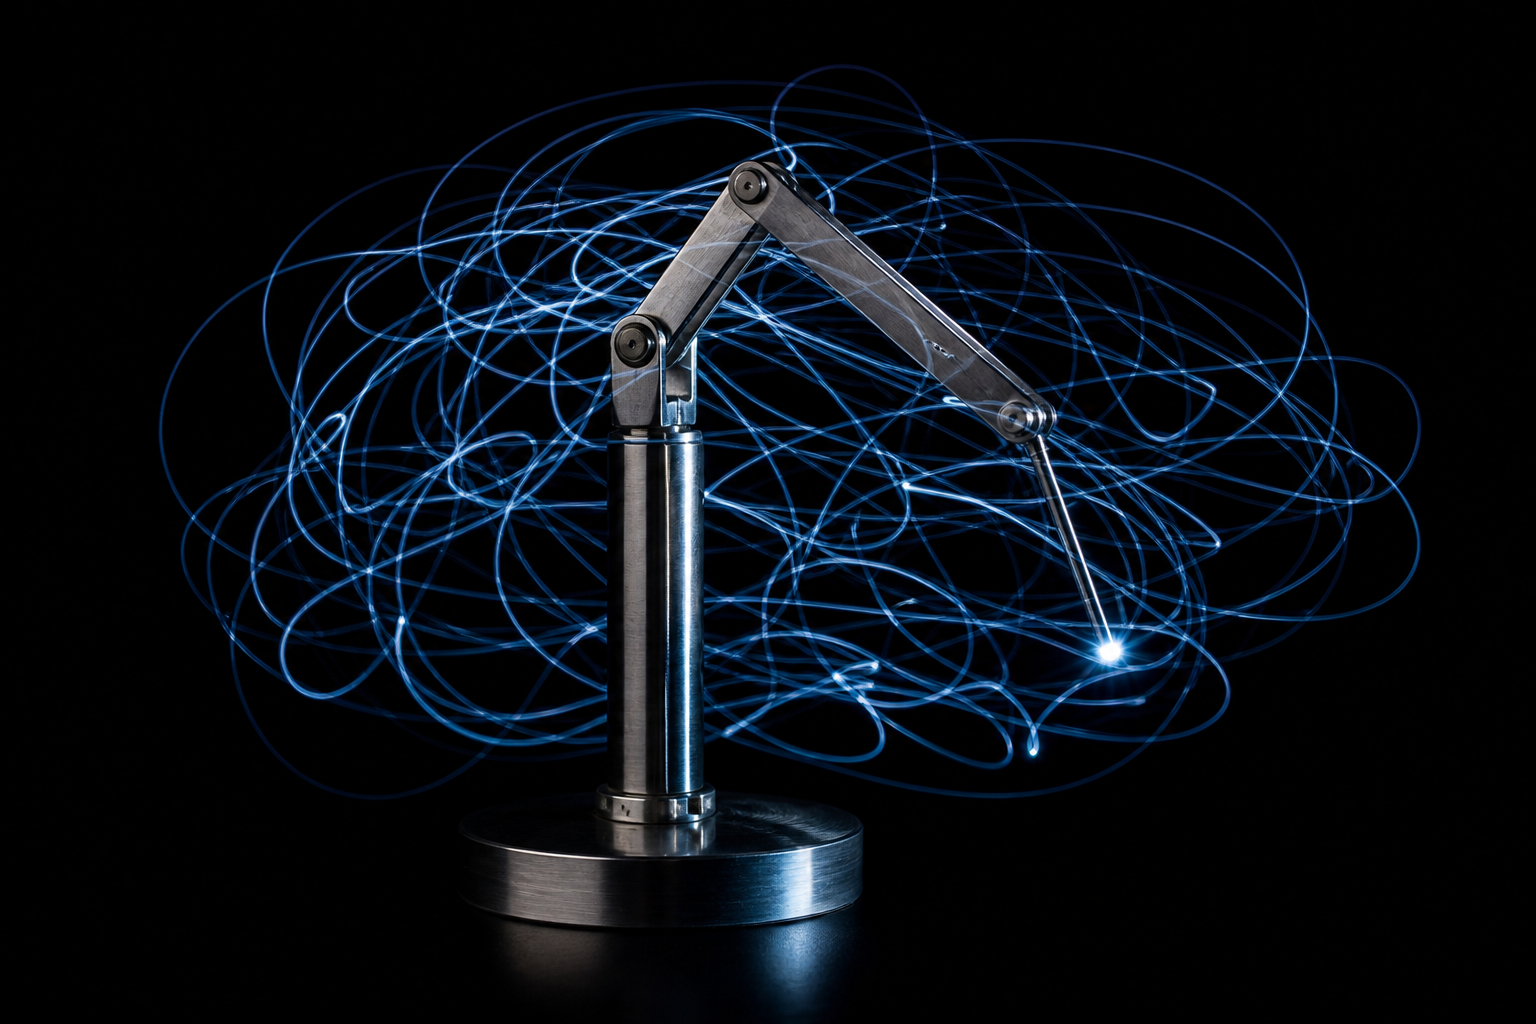
\includegraphics[width=0.58\linewidth]{images/book5/ai/b5-01-double-pendulum-trace.png}

{\small लंबे उद्भासन में खींचा गया द्विक लोलक का पथ: दो निर्देशांक, एक \omterm{def:b3:lagrangian-mechanics:action}{लाग्रांजियन}, और ऐसी गति जिसकी दूर तक भविष्यवाणी कोई सूत्र नहीं करता --- इस अध्याय की न्यूनतम-क्रिया मशीनरी समीकरण लिख देती है; अराजकता उनके हलों को विनम्र बनाए रखती है।}
\end{omfigure}

\section{अभ्यास}

\begin{exercise}[$\star$]\label{exo:b3:lagrangian-mechanics:1}
\omterm{def:b3:lagrangian-mechanics:coordinates}{स्वातंत्र्य कोटि} गिनिए और \omterm{def:b3:lagrangian-mechanics:coordinates}{व्यापकीकृत निर्देशांक} सुझाइए: (क) किसी नियत
कटोरे के भीतरी पृष्ठ पर एक कण; (ख) किसी नियत आनत तल पर बिना फिसले
लुढ़कता बेलन; (ग) ऐसा द्विक लोलक जिसका ऊपरी धुरी-बिंदु किसी क्षैतिज
पटरी पर सरकता है; (घ) अंतरिक्ष में एक डंबल (दो द्रव्यमान, दृढ़ छड़);
(ङ) एक ही नियत वृत्ताकार तार पर दो मनके। इस सूची का कौन-सा \omterm{def:b3:lagrangian-mechanics:coordinates}{प्रतिबंध}
स्थितियों के बजाय वेगों को जोड़ता है, और फिर भी वह होलोनॉमिक रूप में
समाकलनीय क्यों है?
\end{exercise}

\begin{exercise}[$\star$]\label{exo:b3:lagrangian-mechanics:2}
समतलीय लोलक के लिए (\cref{ex:b3:lagrangian-mechanics:pendulum}):
(क) $L$ की और $p_\theta =
\partial L/\partial\dot\theta$ की विमाएँ जाँचिए; (ख) $p_\theta$ को
भौतिक रूप से पहचानिए; (ग) लघु-कोण आवर्तकाल निकालिए; (घ) एक पूरे \omterm{prop:b3:lagrangian-mechanics:modes}{लघु
दोलन} की \omterm{def:b3:lagrangian-mechanics:action}{क्रिया} $S$ निकालिए, जिसका आयाम $\theta_0$ हो --- और गणना करने
से पहले उत्तर की व्याख्या कीजिए (हरात्मक दोलन के लिए $E_k - E_p$ का
समय-औसत क्या होता है?)।
\end{exercise}

\begin{exercise}[$\star$]\label{exo:b3:lagrangian-mechanics:3}
एक एटवुड मशीन: द्रव्यमान $m_1$ और $m_2$ किसी आदर्श डोरी से, एक
द्रव्यमानहीन घिरनी के ऊपर से लटके हैं। (क) एक निर्देशांक चुनकर $L$
लिखिए। (ख) त्वरण ज्ञात कीजिए। (ग) न्यूटन की विधि को तनाव चाहिए था ---
वह कहाँ चला गया? (घ) गति ज्ञात हो जाने पर तनाव आप कैसे पुनः प्राप्त
करेंगे?
\end{exercise}

\begin{exercise}[$\star$]\label{exo:b3:lagrangian-mechanics:4}
बेलनाकार निर्देशांकों में एक स्वतंत्र कण: $L = \tfrac12 m(\dot r^2 +
r^2\dot\varphi^2 + \dot z^2)$। (क) कौन-से निर्देशांक चक्रीय हैं, और
संरक्षित संवेग क्या हैं? (ख) कोई बल न लगने पर भी $p_r$ संरक्षित क्यों
\emph{नहीं} है? (ग) $r$ के लिए \omterm{thm:b3:lagrangian-mechanics:euler-lagrange}{ऑयलर--लाग्रांज समीकरण} लिखिए और पद
$mr\dot\varphi^2$ की व्याख्या कीजिए। (घ) जाँचिए कि अचर चाल से तय की गई
सरल रेखा उसे संतुष्ट करती है।
\end{exercise}

\begin{exercise}[$\star\star$]\label{exo:b3:lagrangian-mechanics:5}
द्रव्यमान $m$ का एक गुटका किसी फाँक के घर्षणहीन फलक (कोण $\alpha$) पर
सरकता है; फाँक का द्रव्यमान $M$ है और वह स्वयं घर्षणहीन फर्श पर सरकने
को स्वतंत्र है। (क) दो निर्देशांक चुनिए: फाँक का भुज $X$ और फलक पर नीचे
की ओर गुटके की दूरी $s$; $L$ लिखिए। (ख) कौन-सा निर्देशांक चक्रीय है,
और वह कौन-सा संरक्षण नियम व्यक्त करता है? (ग) दोनों त्वरण ज्ञात कीजिए।
(घ) सीमाएँ $M \to \infty$ और $\alpha \to
90^\circ$ जाँचिए।
\end{exercise}

\begin{exercise}[$\star\star$]\label{exo:b3:lagrangian-mechanics:6}
गोलीय लोलक: लंबाई $\ell$ की छड़ पर एक गोलक, दोनों कोणों में स्वतंत्र
($\theta$ नीचे की ऊर्ध्वाधर से, $\varphi$ उसके परितः)। (क)
$L$ लिखिए। (ख) \omterm{def:b3:lagrangian-mechanics:momentum}{चक्रीय निर्देशांक} और संरक्षित
$p_\varphi$ पहचानिए। (ग) $\theta$ की गति को किसी प्रभावी विभव में
समेटिए और उसका रेखाचित्र बनाइए। (घ) शंक्वाकार गति $\theta =
\theta_0$ के लिए वर्ष 1 के खंड का शंक्वाकार-लोलक संबंध $\cos\theta_0 =
g/\ell\omega^2$ पुनः प्राप्त कीजिए।
\end{exercise}

\begin{exercise}[$\star\star$]\label{exo:b3:lagrangian-mechanics:7}
द्रव्यमान $m$, लंबाई $\ell$ का एक लोलक द्रव्यमान $M$ की उस गाड़ी से
लटका है जो किसी क्षैतिज पटरी पर लुढ़कने को स्वतंत्र है। (क) निर्देशांक
$X$ (गाड़ी) और $\theta$ लेकर $L$ लिखिए। (ख) क्या संरक्षित है, और
भौतिक रूप से क्यों? (ग) लघु $\theta$ के लिए रैखिकीकरण कीजिए और दिखाइए
कि दोलन-आवृत्ति $\Omega = \sqrt{(1 + m/M)\,g/\ell}$ है। (घ) सीमाएँ $M \to
\infty$ और $M \to 0$ समझाइए --- हल्की गाड़ी आवृत्ति \emph{बढ़ा} क्यों
देती है?
\end{exercise}

\begin{exercise}[$\star\star$]\label{exo:b3:lagrangian-mechanics:8}
आवेश $q$ का एक कण किसी एकसमान क्षेत्र $\vect B = B\vect e_z$ में,
जिसे $\vect A = \tfrac12\vect B\wedge\vect r$ से वर्णित किया गया है।
(क) कार्तीय निर्देशांकों में $L$ लिखिए। (ख) गति के समीकरण निकालिए और
जाँचिए कि वे $\omega_{\text{c}} = qB/m$ पर साइक्लोट्रॉन वृत्त का वर्णन
करते हैं। (ग) संयुग्मी संवेग $p_x$, $p_y$ निकालिए: क्या वे $m\dot x$,
$m\dot y$ हैं? क्या वे संरक्षित हैं? (घ) दिखाइए कि बेलनाकार
निर्देशांकों में लिखे $L$ में $\varphi$ चक्रीय है, और अक्ष पर केंद्रित
वृत्त के लिए संरक्षित $p_\varphi$ पहचानिए।
\end{exercise}

\begin{exercise}[$\star\star$]\label{exo:b3:lagrangian-mechanics:9}
घूमते वलय पर मनके के लिए
(\cref{ex:b3:lagrangian-mechanics:hoop}): (क) \omterm{prop:b3:lagrangian-mechanics:energy}{ऊर्जा फलन} $h$ निकालिए
और जाँचिए कि गति के समीकरण से वह संरक्षित है; (ख) यांत्रिक ऊर्जा $E$
निकालिए और दिखाइए कि $E - h =
m\omega^2R^2\sin^2\theta$; (ग) मोटर द्वारा दी गई शक्ति को
$\theta$ और $\dot\theta$ के फलन के रूप में ज्ञात कीजिए; (घ) जब
$\omega^2 > g/R$ हो, तब झुकी हुई साम्यावस्था के परितः लघु दोलनों की
आवृत्ति ज्ञात कीजिए, और दिखाइए कि $\omega^2 \to g/R$ होने पर वह लुप्त
हो जाती है --- यही वह मंदन है जो कूप के विभाजन की घोषणा करता है।
\end{exercise}

\begin{exercise}[$\star\star\star$]\label{exo:b3:lagrangian-mechanics:10}
समान द्विक लोलक ($m_1 = m_2 = m$, $\ell_1 = \ell_2 = \ell$)।
(क) दिखाइए कि लघु कोणों के लिए $L = \tfrac12 m\ell^2(2\dot\theta_1^2 +
2\dot\theta_1\dot\theta_2 + \dot\theta_2^2) - \tfrac12 mg\ell(2
\theta_1^2 + \theta_2^2)$। (ख) गति के दोनों समीकरण लिखिए। (ग)
प्रसामान्य आवृत्तियाँ $\Omega_\pm^2 = (2 \mp \sqrt2)\,g/\ell$ और
हर विधा का आकार ($\theta_2 = \pm\sqrt2\,\theta_1$) ज्ञात कीजिए। (घ)
बड़े आयाम पर यह तंत्र अराजकता का मानक उदाहरण है: कुछ पंक्तियों में
समझाइए कि लघु-कोण विश्लेषण किस कारण टूटता है, और कोई संरक्षण नियम
क्यों नहीं खोता।
\end{exercise}

\begin{exercise}[$\star\star\star$]\label{exo:b3:lagrangian-mechanics:11}
\emph{ब्रैकिस्टोक्रोन।} एक मनका मूल बिंदु पर विराम से, बिना घर्षण के,
किसी वक्र $y(x)$ ($y$ नीचे की ओर) पर सरककर बिंदु $(a, b)$ तक जाता है।
(क) ऊर्जा-संरक्षण से दिखाइए कि उतरने का समय $T =
\int_0^a\sqrt{(1 + y'^2)/2gy}\,\dd x$ है --- एक फलनक, जिसमें $x$
समय की भूमिका निभाता है। (ख) समाकल्य $F(y, y')$ में स्पष्ट
$x$ नहीं है: दिखाइए कि $h = y'\,\partial F/\partial y' - F$ इष्टतम वक्र
के अनुदिश अचर है (वही गणना जो
\cref{prop:b3:lagrangian-mechanics:energy} में है)। (ग) निष्कर्ष
निकालिए कि $y(1 + y'^2) =
2r$, जहाँ $r$ कोई अचर है, और जाँचिए कि चक्रज $x = r(\phi -
\sin\phi)$, $y = r(1 - \cos\phi)$ उसे संतुष्ट करता है। (घ) दिखाइए कि
एक चाप के तल तक उतरने में मनके को $\pi\sqrt{r/g}$ लगता है, और उसकी
तुलना उसी बिंदु तक की सीधी ढलान से कीजिए।
\end{exercise}

\begin{exercise}[$\star\star\star$]\label{exo:b3:lagrangian-mechanics:12}
\emph{फ़र्मा, \omterm{thm:b3:lagrangian-mechanics:euler-lagrange}{न्यूनतम क्रिया} के रूप में।} अपवर्तनांक $n(y)$ के किसी
माध्यम में प्रकाश दो बिंदुओं के बीच न्यूनतम समय में चलता है (वर्ष 2 का
खंड)। (क) दिखाइए कि $y(x)$ के अनुदिश यात्रा-काल $T = \tfrac1c\int n(y)\sqrt{1 +
y'^2}\,\dd x$ है। (ख) चूँकि समाकल्य में स्पष्ट $x$ नहीं है, पिछले
अभ्यास के संरक्षित $h$ से दिखाइए कि $n(y)\big/\sqrt{1 +
y'^2} = \text{अचर}$, और जाँचिए कि ऊर्ध्वाधर से नापी गई किरण के लिए यही
स्नेल का नियम $n\sin i =
\text{अचर}$ है। (ग) किसी तपती सड़क के ऊपर
अपवर्तनांक ऊँचाई के साथ $n(y) \approx n_0(1 + \beta y)$ की तरह बढ़ता है;
दिखाइए कि लगभग क्षैतिज किरण वक्रता-त्रिज्या $R \approx
1/\beta$ से मुड़ती है। (घ) $\beta = \qty{1.2e-5}{m^{-1}}$ के लिए, सड़क
से \qty{1.2}{m} ऊपर आँखों वाला चालक कितनी दूर से उस पर
``पानी'' की मरीचिका देखता है?
\end{exercise}

\begin{omfigure}
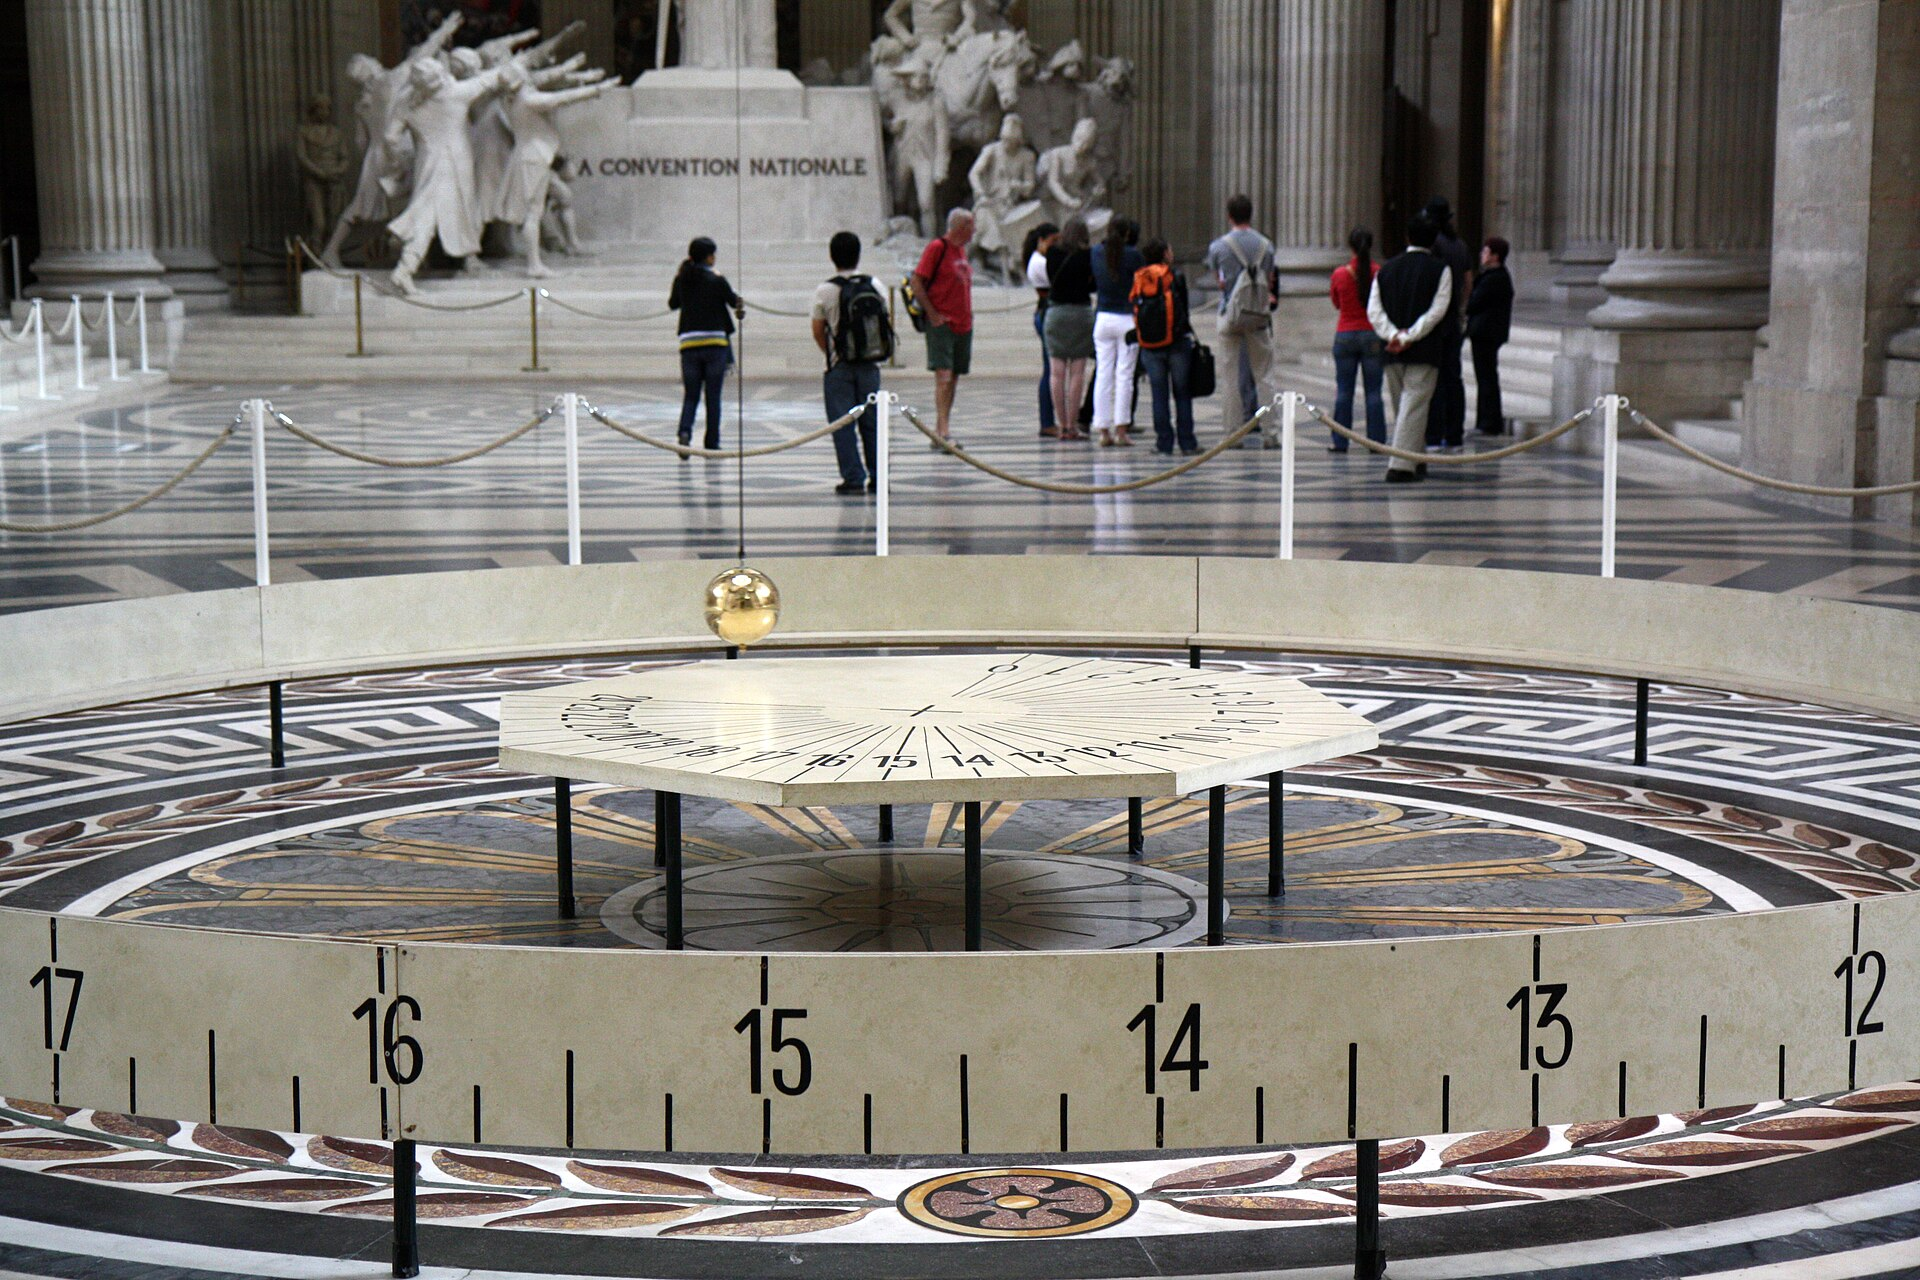
\includegraphics[width=0.6\linewidth]{images/book5/photo-foucault-pantheon.jpg}

{\small पेरिस के पैंथियन में फूको का लोलक। \omterm{def:b3:lagrangian-mechanics:coordinates}{व्यापकीकृत निर्देशांक}, एक \omterm{def:b3:lagrangian-mechanics:coordinates}{प्रतिबंध}, और धीरे-धीरे घूमता एक निर्देश तंत्र: कमरे का घूर्णन गति के समीकरणों में प्रकट होता है --- और झूलने के तल का खिसकना किसी तहखाने को पृथ्वी का घूर्णन नाप लेने देता है। छायाचित्र: ओल्गा ख़ोमित्सेविच, CC~BY~2.0.}
\end{omfigure}

\section{समस्या: वह झाड़ू जो उलटी खड़ी रहती है}

\begin{problem}[{सप्ताहांत समस्या --- कपित्सा का उलटा लोलक}]\label{pb:b3:lagrangian-mechanics:1}
कोई दृढ़ लोलक अपने धुरी-बिंदु के \emph{ऊपर} स्थायी रूप से खड़ा रह सकता
है, बशर्ते धुरी-बिंदु को ऊपर-नीचे पर्याप्त तेज़ी से हिलाया जाए --- यह
विश्लेषण कपित्सा ने 1951 में किया, जो देखने में जादू का खेल लगता है और
जिस सिद्धांत से दोलायमान विद्युत् क्षेत्र एकल आयनों को बाँध लेते हैं।
हम लोलक का निदर्शन इस तरह करते हैं: एक बिंदु-द्रव्यमान $m$, जो लंबाई
$\ell = \qty{40}{cm}$ की द्रव्यमानहीन दृढ़ छड़ के सिरे पर है; $\theta$
\emph{नीचे की} ऊर्ध्वाधर से नापा गया कोण है; $g = \qty{9.81}{m/s^2}$।

\medskip\noindent\textbf{भाग I --- दृढ़ लोलक।}
पहले धुरी-बिंदु को स्थिर रखा जाता है।
\begin{enumerate}
  \item \omterm{def:b3:lagrangian-mechanics:action}{लाग्रांजियन} और गति का समीकरण लिखिए।
  \item लघु दोलनों की आवृत्ति $f_0$ दीजिए, जो $\theta =
        0$ के परितः हों, और उसका मान भी।
  \item दिखाइए कि यहाँ $h = E$ है, और उसके संरक्षण से गोलक की वह
        न्यूनतम प्रक्षेप-चाल ज्ञात कीजिए, तल पर, जो उसे शीर्ष तक
        पहुँचा दे।
  \item $\theta = \pi$ के निकट समीकरण का रैखिकीकरण कीजिए ($\theta = \pi +
        \epsilon$ रखिए) और दिखाइए कि $\ddot\epsilon = +(g/\ell)\epsilon$:
        एक मिलिडिग्री का प्रारंभिक झुकाव कितनी तेज़ी से बढ़ता है? उसे
        $e$ गुना बढ़ने में लगने वाला समय दीजिए।
  \item उँगली की नोक पर सधी झाड़ू लगभग एक सेकंड में गिर जाती है, फिर भी
        अपने आप कभी खड़ी नहीं रहती: एक वाक्य में बताइए कि रैखिकीकृत
        समीकरण साम्यावस्था $\theta = \pi$ के विषय में क्या कहता है।
\end{enumerate}

\medskip\noindent\textbf{भाग II --- धुरी-बिंदु को हिलाना।}
अब धुरी-बिंदु ऊर्ध्वाधर दिशा में दोलन करता है, उसकी ऊँचाई $y_{\text{s}}(t) =
a\cos\Omega t$, जहाँ $a = \qty{2.0}{cm}$ और $\Omega$ समायोज्य है।
\begin{enumerate}[resume]
  \item गोलक के निर्देशांक लिखिए और दिखाइए कि
        $\vect v^{\,2} = \ell^2\dot\theta^2 -
        2a\Omega\ell\sin(\Omega t)\sin\theta\,\dot\theta +
        a^2\Omega^2\sin^2\Omega t$।
  \item दिखाइए कि किसी पूर्ण समय-अवकलज $\dd F(q,t)/\dd t$ जितने भिन्न
        दो \omterm{def:b3:lagrangian-mechanics:action}{लाग्रांजियन} एक ही \omterm{thm:b3:lagrangian-mechanics:euler-lagrange}{ऑयलर--लाग्रांज समीकरण} देते हैं।
  \item इस स्वतंत्रता का उपयोग करके \omterm{def:b3:lagrangian-mechanics:action}{लाग्रांजियन} को $L = \tfrac12 m
        \ell^2\dot\theta^2 - ma\Omega^2\ell\cos(\Omega t)\cos\theta +
        mg\ell\cos\theta$ तक सरल कीजिए। (संकेत:
        $\sin(\Omega t)\sin\theta\,\dot\theta$ किसी
        $\cos(\Omega t)\cos\theta$ पद के साथ मिलकर पूर्ण अवकलज बन जाता
        है; केवल $t$ पर निर्भर पद छोड़े जा सकते हैं।)
  \item गति का समीकरण
        \[
        \ddot\theta = -\frac{g}{\ell}\sin\theta
         + \frac{a\Omega^2}{\ell}\cos(\Omega t)\sin\theta .
        \]
        निकालिए। दूसरे पद की व्याख्या इस रूप में कीजिए कि भार का स्थान $g +
        \ddot y_{\text{s}}$ ले लेता है: लोलक किसी लिफ़्ट में रहता है।
  \item क्या अब \omterm{prop:b3:lagrangian-mechanics:energy}{ऊर्जा फलन} $h$ संरक्षित है? क्या ऊर्जा संरक्षित है?
        ऊर्जा भीतर-बाहर कौन पहुँचाता है?
  \item कपित्सा के परिसर में $a \ll \ell$ और $\Omega \gg \omega_0 =
        \sqrt{g/\ell}$: $a = \qty{2}{cm}$, $\ell =
        \qty{40}{cm}$, $\Omega/2\pi = \qty{40}{Hz}$ के लिए ये जाँचिए,
        और भौतिक रूप से समझाइए कि तब गोलक चालक-दोलन का अनुसरण क्यों
        नहीं कर पाता।
\end{enumerate}

\medskip\noindent\textbf{भाग III --- तेज़ को धीमे से अलग करना।}
गति को $\theta(t) = \Theta(t) + \xi(t)$ के रूप में खोजिए: एक धीमा
अपवाह $\Theta$ और उस पर चालक-आवृत्ति की एक छोटी लहर $\xi$।
\begin{enumerate}[resume]
  \item हर पक्ष का केवल सबसे बड़ा पद रखते हुए दिखाइए कि लहर
        $\ddot\xi \approx +(a\Omega^2/\ell)\cos(\Omega t)
        \sin\Theta$ का पालन करती है, जहाँ चालक की समय-मापनी पर
        $\Theta$ जमा हुआ मान लिया गया है।
  \item $\xi(t) = -(a/\ell)\cos(\Omega t)\sin\Theta$ निकालिए, और
        जाँचिए कि उसका आयाम छोटा है, $a/\ell$ की कोटि का।
  \item $\sin\theta = \sin(\Theta + \xi)$ का $\xi$ में प्रथम कोटि तक
        प्रसार कीजिए और उसे गति के समीकरण में रखिए।
  \item $\Theta$ को स्थिर रखते हुए एक चालक-आवर्तकाल पर औसत लीजिए;
        $\langle\cos\Omega t\rangle = 0$ और
        $\langle\cos^2\Omega t\rangle = \tfrac12$ का उपयोग करके दिखाइए
        कि
        \[
        \ddot\Theta = -\frac{g}{\ell}\sin\Theta
         - \frac{a^2\Omega^2}{2\ell^2}\sin\Theta\cos\Theta .
        \]
  \item दिखाइए कि यह \omterm{ex:b3:lagrangian-mechanics:hoop}{प्रभावी स्थितिज ऊर्जा}
        \[
        U_{\text{प्र}}(\Theta) = mg\ell\Big({-\cos\Theta}
         + \frac{a^2\Omega^2}{4g\ell}\sin^2\Theta\Big) .
        \]
        में गति है।
  \item घूमते वलय पर मनके से तुलना कीजिए
        (\cref{ex:b3:lagrangian-mechanics:hoop}): गणित वही है, नए पद
        का चिह्न उलटा --- हिलाना \emph{तल} की साम्यावस्था के साथ वह
        क्या करता है जो घूर्णन ने नहीं किया?
  \item मंद और द्रुत चालन के लिए $U_{\text{प्र}}$ का रेखाचित्र बनाइए,
        और दोनों स्थितियों में हर साम्यावस्था तथा उसका स्थायित्व
        बताइए।
\end{enumerate}

\medskip\noindent\textbf{भाग IV --- झाड़ू खड़ी हो जाती है।}
\begin{enumerate}[resume]
  \item $U_{\text{प्र}}$ का $\Theta = \pi$ के निकट प्रसार करके दिखाइए
        कि उलटी स्थिति ठीक तभी स्थायी होती है जब
        \[
        a^2\Omega^2 > 2g\ell .
        \]
  \item हमारे लोलक के लिए क्रांतिक चालक-आवृत्ति $f_{\text{c}} =
        \Omega_{\text{c}}/2\pi$ निकालिए, तथा वह शिखर धुरी-चाल
        $a\Omega_{\text{c}}$ और त्वरण $a\Omega_{\text{c}}^2$ ($g$ के
        मात्रकों में) जिनकी वह माँग करती है।
  \item $\Omega = 2\Omega_{\text{c}}$ पर खड़े लोलक के $\Theta = \pi$ के
        परितः धीमे झूलने की आवृत्ति और उसका मान ज्ञात कीजिए; जाँचिए कि
        वह वास्तव में चालन की तुलना में धीमी है।
  \item $\Omega = 2\Omega_{\text{c}}$ पर ही, लहर का आयाम $\xi$ कितना है
        --- $\Theta$ के $\pi$ से थोड़ा हटे होने पर, डिग्री में,
        $a/\ell = 0.05$ के लिए? क्या कोई छायाचित्र इस चाल को पकड़ लेगा?
  \item झाड़ू ऊर्ध्वाधर से कितना झुककर भी लौट सकती है? दिखाइए कि खड़ा
        रखने वाला कूप $|\Theta - \pi| <
        \arccos(2g\ell/a^2\Omega^2)$ तक फैला है, और उसे $\Omega =
        2\Omega_{\text{c}}$ पर आँकिए।
  \item स्थिर उँगली की नोक पर झाड़ू सधाता बाज़ीगर भी उसे खड़ा रखता है
        --- पर किस बिलकुल भिन्न क्रियाविधि से? कपित्सा के लोलक की वह
        विशेषता बताइए जिसे किसी पुनर्भरण की आवश्यकता नहीं।
  \item नामित परिणाम का सार लिखिए: \qty{2}{cm} आयाम से \qty{45}{Hz} पर
        --- क्रांतिक आवृत्ति से दुगुनी पर --- हिलाया गया धुरी-बिंदु
        \qty{40}{cm} के लोलक को उलटा खड़ा रखता है, ऐसे कूप में जो
        ऊर्ध्वाधर से लगभग $75^\circ$ तक जाता है, और जिसमें वह लगभग
        \qty{1.4}{Hz} पर धीरे-धीरे झूलता है। भौतिकी में यही औसतन बाँधने
        वाली युक्ति एकल आवेशित कण को रोके रखने के लिए कहाँ काम में लाई
        जाती है?
\end{enumerate}
\end{problem}
